% !TEX root = ../main.tex

%************************************************
\chapter{Outflows and hot dust emission}
\label{ch:sed}

%************************************************

\section{Introduction}

Many quasars and AGN show an excess in their rest-frame near-infrared continuum emission.
This feature is generally attributed to thermal emission from dust heated by optical/ultra-violet radiation from the accretion disc.
The wavelength of the feature ($\sim2$\,$\mu$m) corresponds to the spectral peak for graphite dust at its sublimation temperature \citep[$T\sim1500$\,K;][]{barvainis87}.
This suggests that the hot dust is very close to the central source, at a radius set by the sublimation temperature of the dust grains.
In nearby AGN, reverberation measurements suggest that this radius is a few tens of light days \citep[e.g.][]{minezaki04,suganuma06}, placing the hot dust at the innermost edge of the putative torus-like structure.

Studies have fitted the near-infrared SEDs of AGN using a blackbody spectrum to represent emission from hot dust \citep[e.g.][]{edelson86,barvainis87,kishimoto07,mor09,riffel09,deo11,landt11,mor11,roseboom13}.
A hot dust component is present in the vast majority of AGN, although populations of `dust-free' objects have also been uncovered \citep{hao10,hao11,jiang10,mor11}.
It is not yet clear how hot dust properties including the temperature and covering factor relate to other AGN properties such as BH mass, luminosity and accretion rate.

In recent years, the picture of the dusty torus has evolved away from a static `doughnut' towards a more general circum-nuclear, geometrically and optically thick dust distribution.
As we have previously discussed (Section~\ref{sec:ch1-winds}), winds and outflows launched from the accretion disc are very common in AGN.
In the dusty wind model -- first proposed by \citet{konigl94} and later developed by, amongst others, \citet{everett05}, \citet{elitzur06}, \citet{keating12} -- the torus is the dusty part of an accretion disc wind that extends beyond the dust sublimation radius.
The dusty clouds are uplifted above the disc where they are directly exposed to radiation from the central engine.
The dust is heated, and radiates in the near-infrared band.
At the same time, radiation pressure on dust can efficiently accelerate the wind \citep[e.g.][]{fabian12}.
The wind is roughly polar, and so naturally provides circum-nuclear obscuration around the accretion disc and dust-free BLR.
This model is supported by recent interferometric observations of nearby Seyfert galaxies which find that the mid-infrared emission is dominated by dust in the polar regions \citep[e.g.][]{raban09,honig12,honig13,tristram14,lopez-gonzaga16}.

Studying the relationship between emission from hot dust and outflow diagnostics in the BLR can help place constraints on this dusty wind model \citep[e.g.][]{wang13}.
This is now possible by combing data from the SDSS spectroscopic and photometric surveys with infrared photometric surveys such as UKIDSS and WISE.
At redshifts $2\lesssim z \lesssim3$, SDSS spectra reveal BH masses, accretion rates and diagnostics of the BLR dynamics.
At the same time, the available photometric data provides full ultra-violet to infrared rest-frame coverage of the SED.
In particular, the WISE photometry is sensitive to the $3$\,$\mu$m region of the SED which is dominated by hot dust.

In this chapter, we build a simple parametric SED model that is able to reproduce the median optical to infrared colours of tens of thousands of SDSS AGN at redshifts $1 \lesssim z \lesssim 3$ (Section~\ref{sec:ch5-standardmodel}).
We use this model to measure the hot dust properties of a large sample of $2 < z < 2.7$ quasars for which we have already measured \ion{C}{IV} emission properties, BH masses and Eddington ratios (Section~\ref{sec:ch5-hotdust}).

\section{Data}

\begin{table}
  \footnotesize
  \centering
  \begin{tabular}{lcccc}
    \hline
    Survey & Passband & $\lambda_{\text{Eff}}$ [$\mu$m] & AB offset & $A_{\text{filter}}/E(B-V)$ \\
    \hline
    SDSS & $u$ & $0.3543$ & $ 0.913$ & $4.875$ \\
         & $g$ & $0.4770$ & $-0.081$ & $3.793$ \\
         & $r$ & $0.6231$ & $ 0.169$ & $2.721$ \\
         & $i$ & $0.7625$ & $ 0.383$ & $2.099$ \\
         & $z$ & $0.9134$ & $ 0.542$ & $1.537$ \\
    UKIDSS & $Y$ & $1.0305$ &  $0.641$ & $1.194$ \\
           & $J$ & $1.2483$ &  $0.941$ & $0.880$ \\
           & $H$ & $1.6313$ &  $1.378$ & $0.569$ \\
           & $K$ & $2.2010$ &  $1.897$ & $0.352$ \\
    WISE & $W1$ & $3.4$ & $2.691$ & $0.182$\\
         & $W2$ & $4.6$ & $3.331$ & $0.130$\\
         & $W3$ & $12.0$ & $5.174$ & \\
    \hline
  \end{tabular}
  \caption[{Available photometric data, effective wavelengths of passbands, Vega to AB magnitude offsets and conversions from \ebv\, to passband extinction.}]{Available photometric data, effective wavelengths, $\lambda_{\text{Eff}}$, of passbands, Vega to AB magnitude offsets and conversions from \ebv\, to passband extinction.}
  \label{tab:photometry}
\end{table}

\subsection{SDSS}

We use both spectroscopic and photometric data from the SDSS DR$7$ quasar catalogue.
The SDSS photometric survey obtained images in five broad optical passbands: $u$, $g$, $r$, $i$ and $z$ (Table~\ref{tab:photometry}).
We use point-spread function magnitudes from the catalogue.

\subsection{UKIDSS Large Area Survey}

We use the tenth data release of the UKIDSS Large Area Survey which has observed $\sim 3,200$ deg$^2$ in four near-infrared passbands: $Y$, $J$, $H$ and $K$.
We use `apermag$3$' magnitudes, which are aperture corrected magnitudes in a $2''$ diameter aperture.

\subsection{WISE All-WISE Survey}

WISE mapped the entire sky in four mid-IR passbands: $W1$, $W2$, $W3$ and $W4$.
The WISE AllWISE Data Release (`AllWISE') combines data from the nine-month cryogenic phase of the mission that led to the `AllSky' data release with data from the NEOWISE program \citep{mainzer11}.
We use profile-fitting `mpro' magnitudes.
Only information from the first three WISE passbands are used in this work.

\subsection{Computing Vega-AB magnitude offsets}

Vega magnitudes are used throughout this chapter.
This is the native magnitude system for UKIDSS\footnote{We find that adding $0.08$\,mag to the UKIDSS $Y$ passband magnitudes brings the photometry into better agreement with the SDSS $z$ and UKIDSS $J$ photometry.} and WISE.
SDSS uses an `asinh' magnitude system \citep{lupton99} which is intended to be on the AB system \citep{oke83}.
However, the photometric zero-points are known to be slightly off the AB standard.
The $z$ passband is in error by $0.02$ ($z_{\text{AB}} = z_{\text{SDSS}} + 0.02$)\footnote{http://classic.sdss.org/dr$7$/algorithms/fluxcal.html.}.
The $u$ passband was in error by $0.04$\,dex at the time of DR$7$.
However, the $u$ throughput function has subsequently been updated \citep{doi10} and the zero-point is now consistent with the AB system.

We use synthetic photometry to calculate the AB magnitude of Vega in each passband.
This can then be used to compute zero-point offsets between the Vega and AB magnitude systems.
The mean flux density $f_\lambda(P)$ in a passband defined by a throughput function $P(\lambda)$ is given by:

\begingroup\makeatletter\def\f@size{11}\check@mathfonts
\begin{eqnarray}
\label{eq:flux}
  f_\lambda(P) = \frac {\int P(\lambda)f_\lambda(\lambda)\lambda d\lambda} {\int P(\lambda)\lambda d\lambda}
\end{eqnarray}
\endgroup

\noindent where $f_\lambda(\lambda)$ is the flux density of the object.
The passband magnitude is then given by:

\begingroup\makeatletter\def\f@size{11}\check@mathfonts
\begin{eqnarray}
\label{eq:mag}
  m_\lambda(P) & = & -2.5\text{log}(f_\lambda(P)) - m_0(P),
\end{eqnarray}
\endgroup

\noindent where $m_0(P)$ is the zero-point magnitude of passband $P$, given by evaluating Equation~\ref{eq:flux} for a reference spectrum.
In the AB system this is a constant spectral flux density of $3631$\,Jy.
In flux per unit wavelength this is:

\begingroup\makeatletter\def\f@size{11}\check@mathfonts
\begin{eqnarray}
  \frac{f_\lambda(\lambda)}{\text{erg}~\text{cm}^{-2}~\text{s}^{-1} \text{\AA}^{-1}} = 0.1087 \left(\frac{\lambda}{\text{\AA}}\right)^{-2}.
\end{eqnarray}
\endgroup

\noindent In the Vega system, a spectrum of the A$0$V star Vega is used.
Although the magnitude of Vega is by design zero in every passband, more recent measurements reveal the star to have a small positive magnitude.
The Vega to AB zero-point conversions given in Table~\ref{tab:photometry} assume Vega to have a magnitude $0.026$.

\subsection{Galactic extinction correction}

$A(u)$, the Galactic extinction in the $u$ passband, is given in the SDSS catalogue.
It is computed using the maps of \citet{schlegel98}.
\citet{schlegel98} calculate the extinction assuming a $z=0$ elliptical galaxy SED and find $A(u)/E(B-V)=5.155$, where \ebv\, is the relative extinction between the $B$ and $V$ passbands.
Quasar and galaxy optical SEDs have very different shapes, and so we re-derived passband extinctions using a $z=1.5$ quasar SED template\footnote{Extinction corrections were derived by Prof. Paul Hewett.}.
Conversions from the selective extinction \ebv\, to the total extinction $A(\lambda)$ in each passband are given in Table~\ref{tab:photometry}.

\subsection{Cross-matching SDSS to UKIDSS and WISE}

There are $105\,783$ objects in the SDSS DR$7$ quasar catalogue.
While WISE mapped virtually the entire sky, the UKIDSS footprint covers approximately one third of the SDSS footprint.
$36\,607$ objects are cross-matched to UKIDSS (with a $2''$ matching radius) and WISE (with a $3$$''$ matching radius).

\subsection{Quasar sample}

We include only the $20\,637$ quasars with $i$ passband magnitudes brighter than $19.1$, i.e. the quasars selected by the main $z<3$ SDSS quasar selection algorithm \citep{richards02}.
We verified that above the $i=19.1$ limit the sample is $95$ per cent complete in all passbands.
BAL quasars are excluded using the \citet{allen11} catalogue.
The \ion{C}{IV} line parameters of these quasars can not be reliably measured.
This leaves $19\,837$  objects in the sample.

We further limit our sample to the redshift range $1 < z < 3$.
Imposing a $z=1$ lower limit on the redshift of our sample ensures that contributions to the SED from quasar host galaxies are negligible.
The completeness of the main SDSS DR$7$ quasar selection algorithm decreases at $z\sim2.75$, and the limited numbers of quasars at higher redshifts sets the upper redshift limit.
The redshift and luminosity distribution of the final sample, containing $12\,934$ quasars, is shown in Figure~\ref{fig:lum_z}.

\begin{figure}
  \centering
  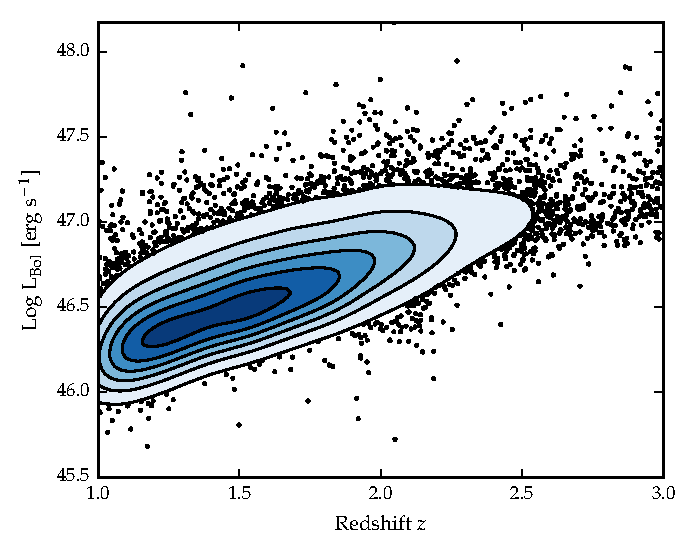
\includegraphics[width=\textwidth]{figures/chapter05/lum_z.pdf}
  \caption[{Distribution of our sample in the redshift-luminosity plane.}]{Distribution of our sample in the redshift-luminosity plane.}
  \label{fig:lum_z}
\end{figure}

\section{Constructing an AGN SED model}

Since the physical processes that power AGN are generally understood only qualitatively, almost all AGN SED templates are empirical.
The empirical template of \citet{elvis94} is still the most commonly cited, despite many additions and updates \citep[e.g.][]{polletta00, kuraszkiewicz03, risaliti04, richards06,  polletta07, lusso10, shang11, marchese12, trichas12}.
However, these composite spectra are often constructed from quasars with a huge range in luminosity as a function of rest-frame wavelength.
In addition, the host-galaxy contribution at optical wavelengths in low-redshift objects can be significant and is challenging to completely eliminate.
There is therefore a strong rationale for taking a parametric approach to modelling quasar SEDs.
This is the approach adopted in this work.

We construct an SED model that is valid between $1216$\,\AA\, and $3$\,$\mu$m.
In this region the SED is dominated by the accretion disc, broad ultra-violet/optical emission-lines and thermal emission from the hottest ($T\sim1200$K) dust.
In this section, we describe how each of these components are represented in our parametric SED model.
The effect of dust extinction at the AGN redshift is also incorporated into the model.
At high redshifts, Ly$\alpha$ forest absorption becomes significant.
Because we do not attempt to include this effect, our model is valid only at wavelengths long-ward of $1216$\,\AA.
We model dust emission using a single temperature ($T\sim1200$\,K) blackbody, which peaks at $\sim2$\,$\mu$m.
At longer wavelengths, emission from cooler dust further from the central engine becomes increasingly important.
We do not include this emission in our model, which restricts its validity to $\lesssim3$\,$\mu$m.
The model spectrum is shown in Figure \ref{fig:modelsed}, with each of the main components indicated.

\begin{figure}[h!]
  \centering
  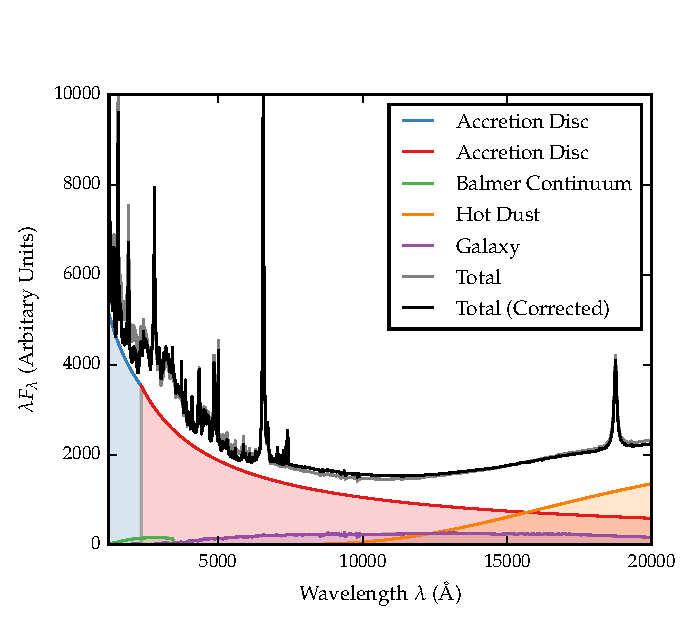
\includegraphics[width=\textwidth]{figures/chapter05/sed_model.pdf}
  \caption[{Model quasar spectrum at $z=1$.}]{Model quasar spectrum at $z=1$, showing the contributions to the total flux from the accretion disc, Balmer continuum, hot dust and emission-lines. }
  \label{fig:modelsed}
\end{figure}

\subsection{Accretion disc}

Thermal accretion disc emission in the $0.1 - 1$\,$\mu$m region is characterised by a broken power-law with three free parameters: a break-wavelength, $\lambda_{\text{break}}$, a blue power-law index, $\alpha_{\text{blue}}$, for wavelengths shorter than the break wavelength, and a red power-law index, $\alpha_{\text{red}}$, for wavelengths longer than the break wavelength \citep[e.g.][]{stevans14}.

\subsection{Balmer continuum}

High order Balmer lines, optically thin Balmer continuum emission, two-photon emission and \ion{Fe}{II} emission blend together to form the `Balmer' continuum at $\sim3000$\,\AA.
We simulate the Balmer continuum using the empirical model given by \citet{grandi82}:

\begingroup\makeatletter\def\f@size{11}\check@mathfonts
\begin{eqnarray}
  F(\lambda) = C_{\text{BC}} \times B_\lambda(T_e)(1-e^{-\tau_\lambda}); \quad \lambda \leq \lambda_{\text{BE}}
\end{eqnarray}
\endgroup

\noindent where $C_{\text{BC}}$ is a normalisation factor, $B_\lambda(T_e)$ is the Planck function, $T_e=13150$\,K is the effective temperature, $\lambda_{\text{BE}}=3460$\,\AA\, is the wavelength at the Balmer edge, and $\tau_\lambda = \tau_{BE}\left( \nicefrac{\lambda_{BE}} {\lambda} \right)^{-3}$ is the optical depth with $\tau_{\text{BE}}=45$ the optical depth at $\lambda_{\text{BE}}$.
This function is convolved with a Gaussian with width $\sigma=5000$\,\kms\, to simulate the effect of bulk velocity shifts comparable to those present in broad AGN emission-lines.
The normalisation factor, $C_{\text{BC}}$, is a free parameter in our model, with the other parameters fixed at the values determined by \citet{grandi82}. 

\subsection{Hot dust}

Thermal emission from hot dust, which dominates the SED at wavelengths longer than $1$\,$\mu$m, is modeled using a blackbody

\begingroup\makeatletter\def\f@size{11}\check@mathfonts
\begin{eqnarray}
  F_\lambda = C_{\text{BB}} \times \frac{2 hc^2}{\lambda^5}\frac{1}{ e^{\frac{hc}{\lambda k_\text{B}T_{\text{BB}}}} - 1},
\end{eqnarray}
\endgroup

\noindent with two free parameters: the temperature $T_{\text{BB}}$ and normalisation $C_{\text{BB}}$ relative to the power-law continuum.

\subsection{Emission-lines}

We use an emission-line template taken from \citet{francis91}, which has been extended by \citet{maddox06} to include the \ha and Pa$\alpha$ emission-lines\footnote{The spectrum is not significantly different from the \citet{vandenberk01} SDSS composite.}.
All emission-lines, with the exception of \ha and \hbns, are scaled equally using a single free parameter $C_{\text{EL}}$, which preserves relative EQWs:

\begingroup\makeatletter\def\f@size{11}\check@mathfonts
\begin{eqnarray}
  F_{\lambda} =  C_{\text{EL}} \times \frac{F_{\lambda, \text{el}}}{F_{\lambda, \text{cont}}} \times F_{\lambda}
\end{eqnarray}
\endgroup

\noindent where $F_{\lambda, \text{el}}$ is the emission-line template, $F_{\lambda,\text{cont}}$ is the continuum flux in the template, and $F_{\lambda}$ is the continuum flux in the SED model.
The redshifts and luminosities of the quasars contributing to the emission-line template change as a function of wavelength.
To account for possible variations in the strengths of the different lines, \ha and \hb are scaled separately with parameter $C_{{\text{H}} \alpha}$:

\begingroup\makeatletter\def\f@size{11}\check@mathfonts
\begin{eqnarray}
  F_{\lambda} =  C_{\text{EL}} \times C_{{\text{H}} \alpha} \times \left( \frac{L(z)} {L(z_{\text{nrm}})} \right)^{\beta} \times \frac{F_{\lambda, \text{el}}}{F_{\lambda, \text{cont}}} \times F_{\lambda}.
\end{eqnarray}
\endgroup

\noindent The luminosity dependence of the \ha and \hb EQW (i.e. the Baldwin effect) is parametrised with a power-law with slope $\beta=-0.04$.
The dependence of the mean AGN luminosity on redshift, $L(z)$, is determined empirically from the SDSS quasar catalogue.

\subsection{Dust extinction}
\label{sec:sed-extinction}

We simulate the effect of dust extinction at the quasar redshift using a custom extinction curve that is appropriate for the quasar population\footnote{The extinction curve has been derived by Prof. Paul Hewett.}.
To derive the quasar extinction curve, UKIDSS photometry was used to provide an \ebv\, estimate, via the magnitude displacement of each quasar from the locus of un-reddened objects.
At redshifts $2 < z < 3$ the reddening measure is made at rest-frame wavelengths $3500-7000$\,\AA, where Galaxy, LMC and SMC\footnote{LMC and SMC: Large and Small Magellanic Clouds.} extinction curves are very similar.
The SDSS spectra of the same objects are then employed to generate an empirical extinction curve in the ultra-violet, down to $1200$\,\AA.
The resulting curve has no $2200$\,\AA\, feature and rises rapidly with decreasing wavelength but is not as steep as the SMC curve.
The extinction curve gives the colour excess $E(\lambda-V)$ relative to the colour excess \ebv\, as a function of wavelength $\lambda$.
The colour excess \ebv\, is related to the extinction in the $V$ passband, $A(V)$, via the ratio $R_V$:

\begingroup\makeatletter\def\f@size{11}\check@mathfonts
\begin{eqnarray}
  R_V = \frac{A(V)}{E(B-V)}
\end{eqnarray}
\endgroup

\noindent where we assume $R_V = 3$.
Hence the extinction at a wavelength lambda $A(\lambda)$ is

\begingroup\makeatletter\def\f@size{11}\check@mathfonts
\begin{eqnarray}
  A(\lambda) = E(B-V) \times \left[ \frac{E(\lambda-V)}{E(B-V)} + R_V \right]
\end{eqnarray}
\endgroup

\noindent where the colour excess \ebv\, is a free parameter in our model.
The attenuation of the flux at a given wavelength is then:

\begingroup\makeatletter\def\f@size{11}\check@mathfonts
\begin{eqnarray}
  F_\lambda = F_\lambda10^{-A(\lambda)/2.5}
\end{eqnarray}
\endgroup

\noindent in the rest-frame of the quasar.

\section{A parametric SED template for the quasar population}
\sectionmark{SED template}
\label{sec:ch5-standardmodel}

In this section we determine a single set of SED model parameters for all $19\,853$ quasars, encompassing a range of redshifts, luminosities, accretion rates and other properties.

\subsection{Fitting procedure}

\begin{figure}
  \centering
  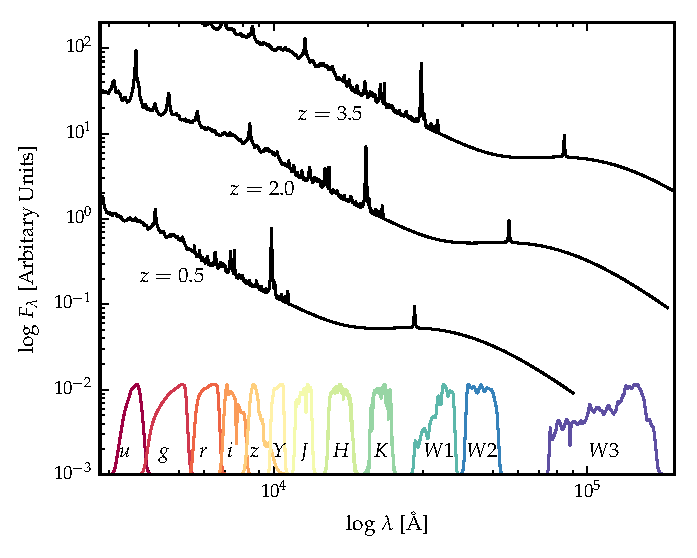
\includegraphics[width=\textwidth]{figures/chapter05/throughput.pdf}
  \caption[{Model quasar spectrum at three different redshifts.}]{Model quasar spectra at three different redshifts and throughput functions for SDSS, UKIDSS and WISE passbands. The model spectra have been offset for clarity.}
  \label{fig:filters}
\end{figure}

The free parameters in our SED model are summarised in Table~\ref{tab:params}.
The reddening \ebv\, is fixed to zero, since a large fraction of SDSS quasars have very small amounts of dust reddening \citep{richards03}.

We divide the quasar sample into redshift bins from $z=1$ to $z=3$ in intervals of $\Delta z = 0.1$.
In each redshift bin median passband magnitudes are calculated, and normalised such that $i=18$.
We use the $rizYJHKW1W2$ passbands to constrain the model, which covers $1550-23000$\,\AA\, in the rest-frame.
Model SEDs are generated at redshifts corresponding to the centres of the redshift bins.
The SED model is shown at three different redshifts in Figure~\ref{fig:filters}.
Model magnitudes are calculated using Equations~\ref{eq:flux} and \ref{eq:mag} and are normalised such that $i=18$.
We find the best-fitting model parameters by minimising the $\chi^2$ statistic for the $9 \times 21 = 189$ model and data magnitudes using the Nelder-Mead algorithm.

\subsection{Quality of fit}

\begin{table}
  \footnotesize
  \centering
  \begin{tabular}{c c c}
    \hline
    Parameter & Symbol & Value \\
    \hline
    Blue power-law index & $\alpha_{\text{blue}}$ & $-0.478$ \\
    Red power-law index & $\alpha_{\text{red}}$ & $-0.199$ \\
    Power-law break & $\lambda_{\text{break}}$ & $2402$ \\
    Blackbody temperature & $T_{\text{BB}}$ & $1306$\,K \\
    Blackbody normalisation & $C_{\text{BB}}$ & $2.673$ \\
    Emission-line scaling & $C_{\text{EL}}$  & $1.240$ \\
    \ha emission-line scaling & $C_{{\text{H}}\alpha}$  & $0.713$ \\
    Balmer continuum scaling & $C_{\text{BC}}$ & $0.135$ \\
    \hline
  \end{tabular}
  \caption[{Free parameters in SED model and best-fitting values from fit to the median colours of quasars at redshifts $1 < z < 3$.}]{Free parameters in SED model and best-fitting values from fit to the median colours of quasars at redshifts $1 < z < 3$.}
  \label{tab:params}
\end{table}

The best-fitting parameters from the fit are given in Table~\ref{tab:params}.
The colours ($r-i$, $i-z$, etc.) of the median SED and the best-fitting model are plotted as a function of redshift in Figure~\ref{fig:color}.
Most of the large variations that can be seen in the median colours as a function of redshift are due to strong emission-lines being redshifted into and out of the passbands.

\begin{figure}
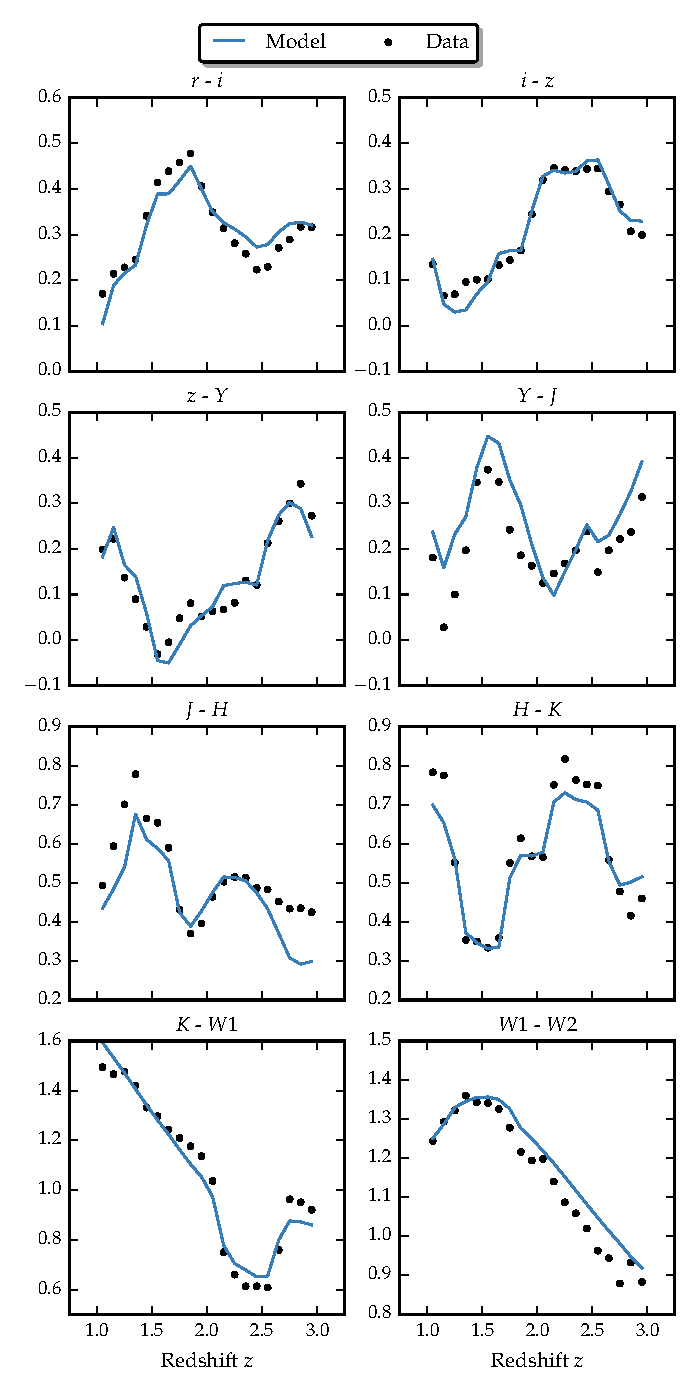
\includegraphics[width=\textwidth]{figures/chapter05/sed_color_plot.pdf}
\caption[{Median colours of quasars and best-fitting SED model as a function of redshift.}]{Median colours of quasars and best-fitting SED model as a function of redshift.}
  \label{fig:color}
\end{figure}

In Figure~\ref{fig:residuals} we show the data minus model residuals as a function of the rest-frame wavelength.
The residuals indicate that over a large redshift range the model is very effective at reproducing the median observed colours of the sample.
Discrepancies are at the $<0.1$\,mag level.
At a given rest-frame wavelength, there are no significant discrepancies between residuals in different passbands.
This indicates that there is no significant evolution in the median SED as a function of redshift.
We conclude that a single, fairly simple parametric model is effective at reproducing the median colours of tens of thousands of AGN with a large dynamic range in redshift and luminosity.

\begin{figure}[t!]
  \centering
  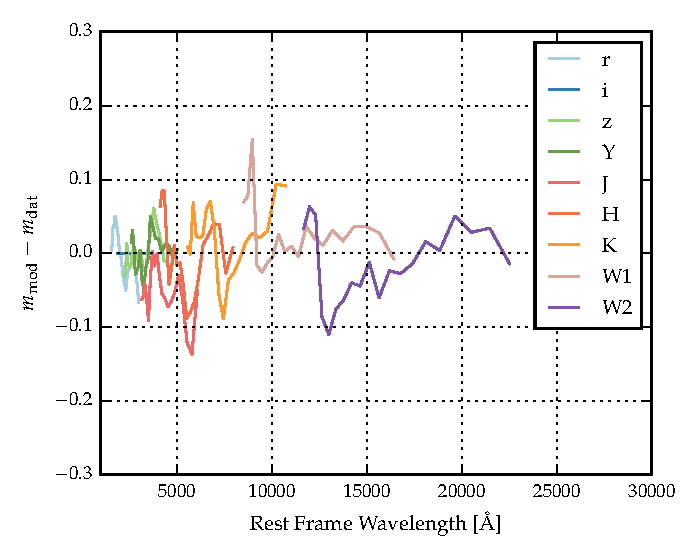
\includegraphics[width=\textwidth]{figures/chapter05/model_residuals.pdf}
  \caption[{Residuals from fitting a single SED model to the colours of $1 < z < 3$ quasars as a function of rest-frame wavelength.}]{Residuals from fitting a single SED model to the colours of $1 < z < 3$ quasars as a function of rest-frame wavelength. Discrepancies are at the $<0.1$\,mag level, demonstrating that a simple parametric model is effective at reproducing the median colours of tens of thousands of AGN with a large dynamic range in redshift and luminosity.}
  \label{fig:residuals}
\end{figure}

\section{Diversity of hot dust properties}
\label{sec:ch5-hotdust}

In Figure~\ref{fig:w1w2colorsratio} we plot the $W1 - W2$ colours of the sample as a function of redshift.
At any given redshift we see a $\sim 0.5$\,mag dispersion in the $W1-W2$ colours.
In this redshift range the $W1$ and $W2$ passbands are probing the $1.2 - 2.8$\,$\mu$m and $1.6 - 3.8$\,$\mu$m regions of the rest frame SED respectively.
The peak wavelength for a blackbody radiating at $1200$\,K is $2.4$\,$\mu$m.
Therefore, the large spread in $W1-W2$ colours is highly suggestive of significant diversity in the hot dust properties in this sample.

We characterise the hot dust properties of our sample in terms of the temperature of the blackbody component and the near-infrared to ultra-violet luminosity ratio, $R_{\text{NIR/UV}}$.
The ultra-violet and near-infrared luminosities are calculated between $2000$ and $9000$\,\AA\, and $1$ and $3$\,$\mu$m respectively in the SED.
We show the $W1-W2$ colours derived from our SED model with a fixed blackbody temperature ($1306$\,K) and varying $R_{\text{NIR/UV}}$ in Figure~\ref{fig:w1w2colorsratio}.
The $W1-W2$ colours indicate that the hot dust luminosity in this sample varies by a factor of $\sim5$.

The temperature is likely related to the distance of the dust from the central engine.
Dust that is closer in will be hotter, with the sublimation temperature of the dust grains setting the minimum radius.
The value of $R_{\text{NIR/UV}}$ may be related to the covering factor of the hot dust.
However, this simple interpretation is somewhat complicated by the fact that at large inclinations sight-lines to the hot dust may be obscured by cooler dust in the putative torus.

In the remainder of this chapter, we will measure hot dust parameters for individual quasars via SED fitting.
We will characterise the range of hot dust properties present in the sample, and test its relation to quasar properties such as luminosity, BH mass and normalised accretion rate, as well as outflow properties.

\begin{figure}[t!]
\centering
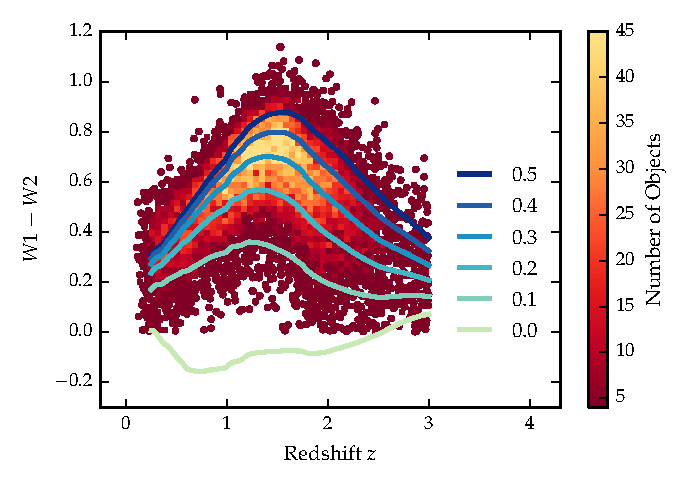
\includegraphics[width=\columnwidth]{figures/chapter05/w1w2_versus_redshift_ratio.pdf}
\caption[{$W1 - W2$ colours of quasars as a function of redshift.}]{$W1 - W2$ colours of quasars as a function of redshift. Above a density threshold of four points per pixel points are represented by a two-dimensional histogram. Overlaid we plot the colours of our SED model, with a fixed blackbody temperature and a varying near-infrared ($1 - 3$\,$\mu$m) to ultra-violet ratio.}
  \label{fig:w1w2colorsratio}
\end{figure}

\subsection{Defining a sample with uniform UV/optical properties}
\label{sec:ch5-hotdustsample}

The shifting of passbands due to redshift limits the redshift range of the quasars for which hot dust properties can be reliably constrained.
Constraining a $T\sim1200$\,K blackbody component in the SED model requires photometric data covering $\sim1-3$\,$\mu$m in the rest-frame of the quasar.
At the limits of the redshift range $2 < z < 2.7$ $W1W2W3$ is probing the $1.1-4$ and $0.9-3.2$\,$\mu$m regions of the SED.
Therefore the available data is sensitive to the hot dust component across the entirety of this redshift interval.
In general, care must be taken looking for trends with luminosity (and related properties including the BH mass and Eddington ratio) given the observed-frame passband information on the rest-frame SED can produce some strong systematics with redshift.
However, the adopted redshift interval is narrow enough to prevent this from being a significant problem in this instance.
In this redshift range, \ion{C}{IV} emission is located within the wavelength coverage of the SDSS spectra.
This will allow us to test the relationship between the hot dust and BLR outflow properties.
There are $2329$ quasars in the sample with redshifts $2 < z < 2.7$.

Holding the rest of the model parameters fixed, we will vary only the parameters of the blackbody.
This requires the SED model to be a reasonable fit to the quasar SEDs in the ultra-violet/optical region.
In practice, this means excluding objects with extreme emission-line EQWs and/or significant dust extinction.
We use $i-K$ as a measure of the overall colour of the quasars as it provides the longest baseline in wavelength without being affected by absorption in the Ly$\alpha$ forest at high redshifts.
$i-K$ colours are shown as a function of redshift in Figure~\ref{fig:ikzplot}.
In the same plot we show the quasar SED model with $E(B-V)=-0.075,\,0,\,0.075$.
A significant amount of the scatter in $i-K$ can be attributed to intrinsic variations in the ultra-violet power-law slopes of the individual quasars.
Because this is degenerate with \ebv, we allow negative \ebv\, values in the SED model.

The SDSS and UKIDSS photometry are separated by $3-4$ years in the source rest-frame.
Therefore, some of the scatter in the $i-K$ colours could be due to temporal variations in the brightness of the targets.
However, the red-asymmetry of the $i-K$ colours about the un-reddened SED model suggests that this effect is sub-dominant to dust extinction.

We discarded from our sample quasars with $i - K$ colours redder than our standard model with dust reddening \ebv $= 0.075$ and bluer than \ebv $=-0.075$ (Figure~\ref{fig:ikzplot}).
Following this cut we are left with $2030$ quasars in the sample.

\begin{figure}[t!]
  \centering
  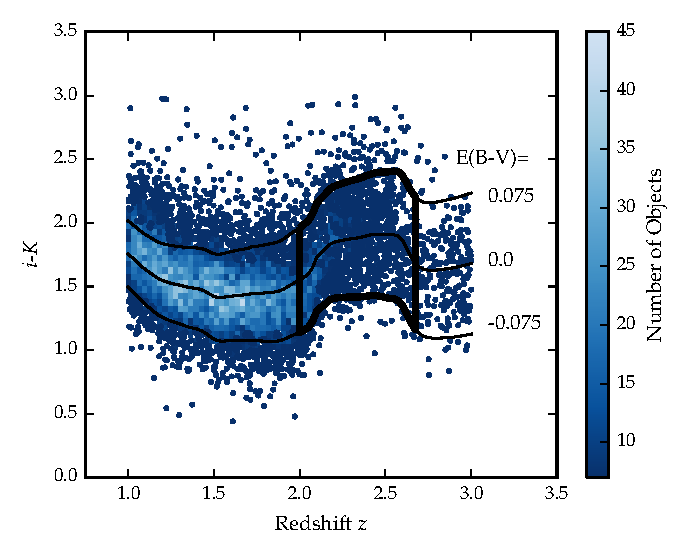
\includegraphics[width=\columnwidth]{figures/chapter05/ik_versus_z_low_ext.pdf}
  \caption[{$i-K$ colours of quasars as a function of redshift.}]{$i-K$ colours of quasars as a function of redshift. The lines show the colours of the SED model with varying amounts of dust extinction. Quasars with extinction $|E(B-V)|>0.075$ are excluded from our $2 < z < 2.7$ sample.}
  \label{fig:ikzplot}
\end{figure}

\subsection{Fitting procedure}

We fit the model to the individual quasar SEDs with the temperature and normalisation of the blackbody component as free parameters.
The model spectrum is redshifted to the redshift of the quasar being fit and passband magnitudes are calculated using Equations~\ref{eq:flux} and \ref{eq:mag}.
We minimise the inverse variance weighted $\chi^2$ statistic using the Levenberg-Marquardt algorithm.
We impose a minimum error of $0.1$\,mag on the quasar magnitudes, corresponding to the size of the residuals from the model fit to the median colours of the population (Figure~\ref{fig:residuals}).
Data from $ugrizYJHKW1W2W3$ is used to constrain the model.
However, to avoid Ly$\alpha$ forest absorption, passbands are excluded if $\lambda_{\text{Eff}} / (1 + z) < 1400$\,\AA.

\subsection{Distribution of hot dust parameters}

The best-fitting hot dust temperature ($T_{\text{BB}}$) and abundance ($R_{\text{NIR/UV}}$) for the individual quasars are shown in Figure~\ref{fig:ratio_tbb_density}.
Even after restricting the sample to have a relative narrow range of ultra-violet/optical SED shapes, we see significant diversity in the hot dust abundance, with the near-infrared to ultra-violet luminosity ratio having a broad range from $0.1$ to $0.6$.
The temperature takes on a relatively narrow range of values: $1177\pm136$\,K.
This is consistent with the dust radius being set by the sublimation temperature of the dust grains.

We note a degeneracy between the temperature and $R_{\text{NIR/UV}}$.
This is a result of the dependence of the blackbody peak on temperature and the fixed wavelength interval used to calculate the blackbody luminosity.
However, this does not affect any of the results presented below.

\begin{figure}[t!]
  \centering
  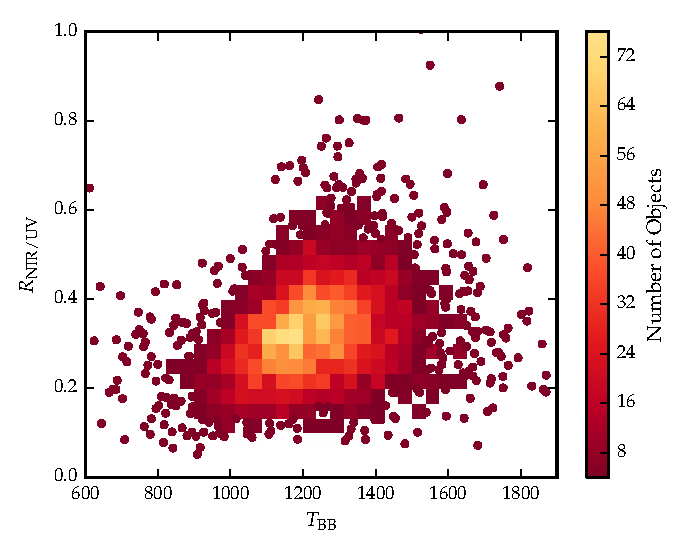
\includegraphics[width=0.9\textwidth]{figures/chapter05/ratio_tbb_density.pdf}
  \caption[{Histograms of the ratio of near-infrared to ultra-violet luminosity and blackbody temperature and the correlation between these two parameters.}]{Histograms of the ratio of near-infrared to ultra-violet luminosity ($R_{\text{NIR/UV}}$) and blackbody temperature ($T_{BB}$) and the correlation between these two parameters. }
  \label{fig:ratio_tbb_density}
\end{figure}

\subsection{Relationship between hot dust and BLR outflows}

\begin{figure}[t!]
\centering
  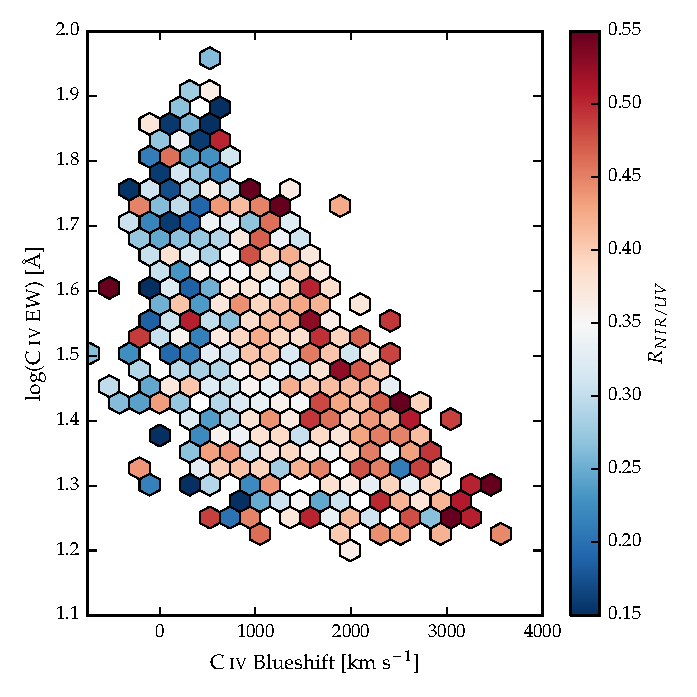
\includegraphics[width=0.9\textwidth]{figures/chapter05/hot_dust_ratio.pdf}
\caption[{Hot dust abundance as a function of rest-frame EQW and blueshift of the \ion{C}{IV} line.}]{Rest-frame EQW and blueshift of the \ion{C}{IV} line. The colours of the hexagons denote the median hot dust ($T\simeq1200$\,K) abundance for all quasars at a given EQW and blueshift. Quasars with the most extreme outflow signatures (in the bottom right) have enhanced hot dust emission.}
  \label{fig:civ_hot_dust}
\end{figure}

In this section, we measure the dependence of the hot dust parameters on the blueshift and EQW of the \ion{C}{IV} emission.
\ion{C}{IV} measurements are described in Section~\ref{sec:ch3-application} and the \ion{C}{IV} blueshift is defined with respect to a systemic redshift measured by Allen \& Hewett (2017, in preparation).
This information is available for $98$ per cent of the objects in our sample.

In Figure~\ref{fig:civ_hot_dust} we show that the near-infrared to ultra-violet luminosity ratio is correlated with the \ion{C}{IV} blueshift and EQW.
There is a clear enhancement in the hot dust emission for quasars in the large \ion{C}{IV} blueshift, low EQW region of the parameter space: for quasars with \ion{C}{IV} blueshifts $>2000$\,\kms, $R_{\text{NIR/UV}}=0.43\pm0.13$, while for quasars with \ion{C}{IV} blueshifts $<1000$\,\kms, $R_{\text{NIR/UV}}=0.31\pm0.14$ (median $\pm$ intra-sample dispersion).
A similar result was recently reported by \citet{wang13}.
The distribution of blackbody temperatures is relatively narrow ($\sigma\sim200$\,K) and so, as expected, we do not observe any correlations between the hot dust temperature and the \ion{C}{IV} emission parameters.

The profiles of the emission-lines with large \ion{C}{IV} blueshifts suggest that the BLR dynamics in these objects are dominated by high-velocity outflows.
As we discussed in the introduction to this chapter, outflows from the outer regions of the accretion disc could contain significant amounts of dust.
As the dusty wind is lifted above the accretion disc, it is directly exposed to ultra-violet radiation from the inner accretion disc.
Radiation pressure could then efficiently accelerate the wind owing to the high cross-section of the dust grains\footnote{Radiation line-driving and free electrons are also likely to play important roles in accelerating the wind.} \citep[e.g.][]{fabian12}.
This would flatten the geometry of the wind, which would expose more of the inner edge of the base of the wind to relatively face-on lines of sight.
This is where the hot dust is located, and so the hot dust emission would be enhanced.
The more the wind is accelerated, the flatter it's geometry will become, and the more hot dust will be exposed.
This model therefore predicts the correlation we observe between the strength of BLR outflows (which is reflected in the \ion{C}{IV} blueshift) and the hot dust abundance.
The geometry of this dusty wind model is illustrated in Figure~\ref{fig:kishimoto}.

The hot dust abundance in $z\lesssim1$ SDSS AGN is also found to be higher when optical \ion{Fe}{II} is strong \citep{shen14}.
Given the known correlations between the \ion{C}{IV} emission properties and the \ion{Fe}{II} strength (e.g. Figures~\ref{fig:ev1_lowz} and \ref{fig:ev1}), this is very likely to be a related result.
Recent results from \citet{roseboom13} reporting an anti-correlation between the torus covering factor and the hot dust abundance are also naturally explained in this model.
If the circum-nuclear obscuration is due to the dusty accretion disc wind, then flattening the geometry of the wind will decrease the torus covering factor and increase the surface area of hot dust that can be seen.

\begin{figure}[t!]
\centering
  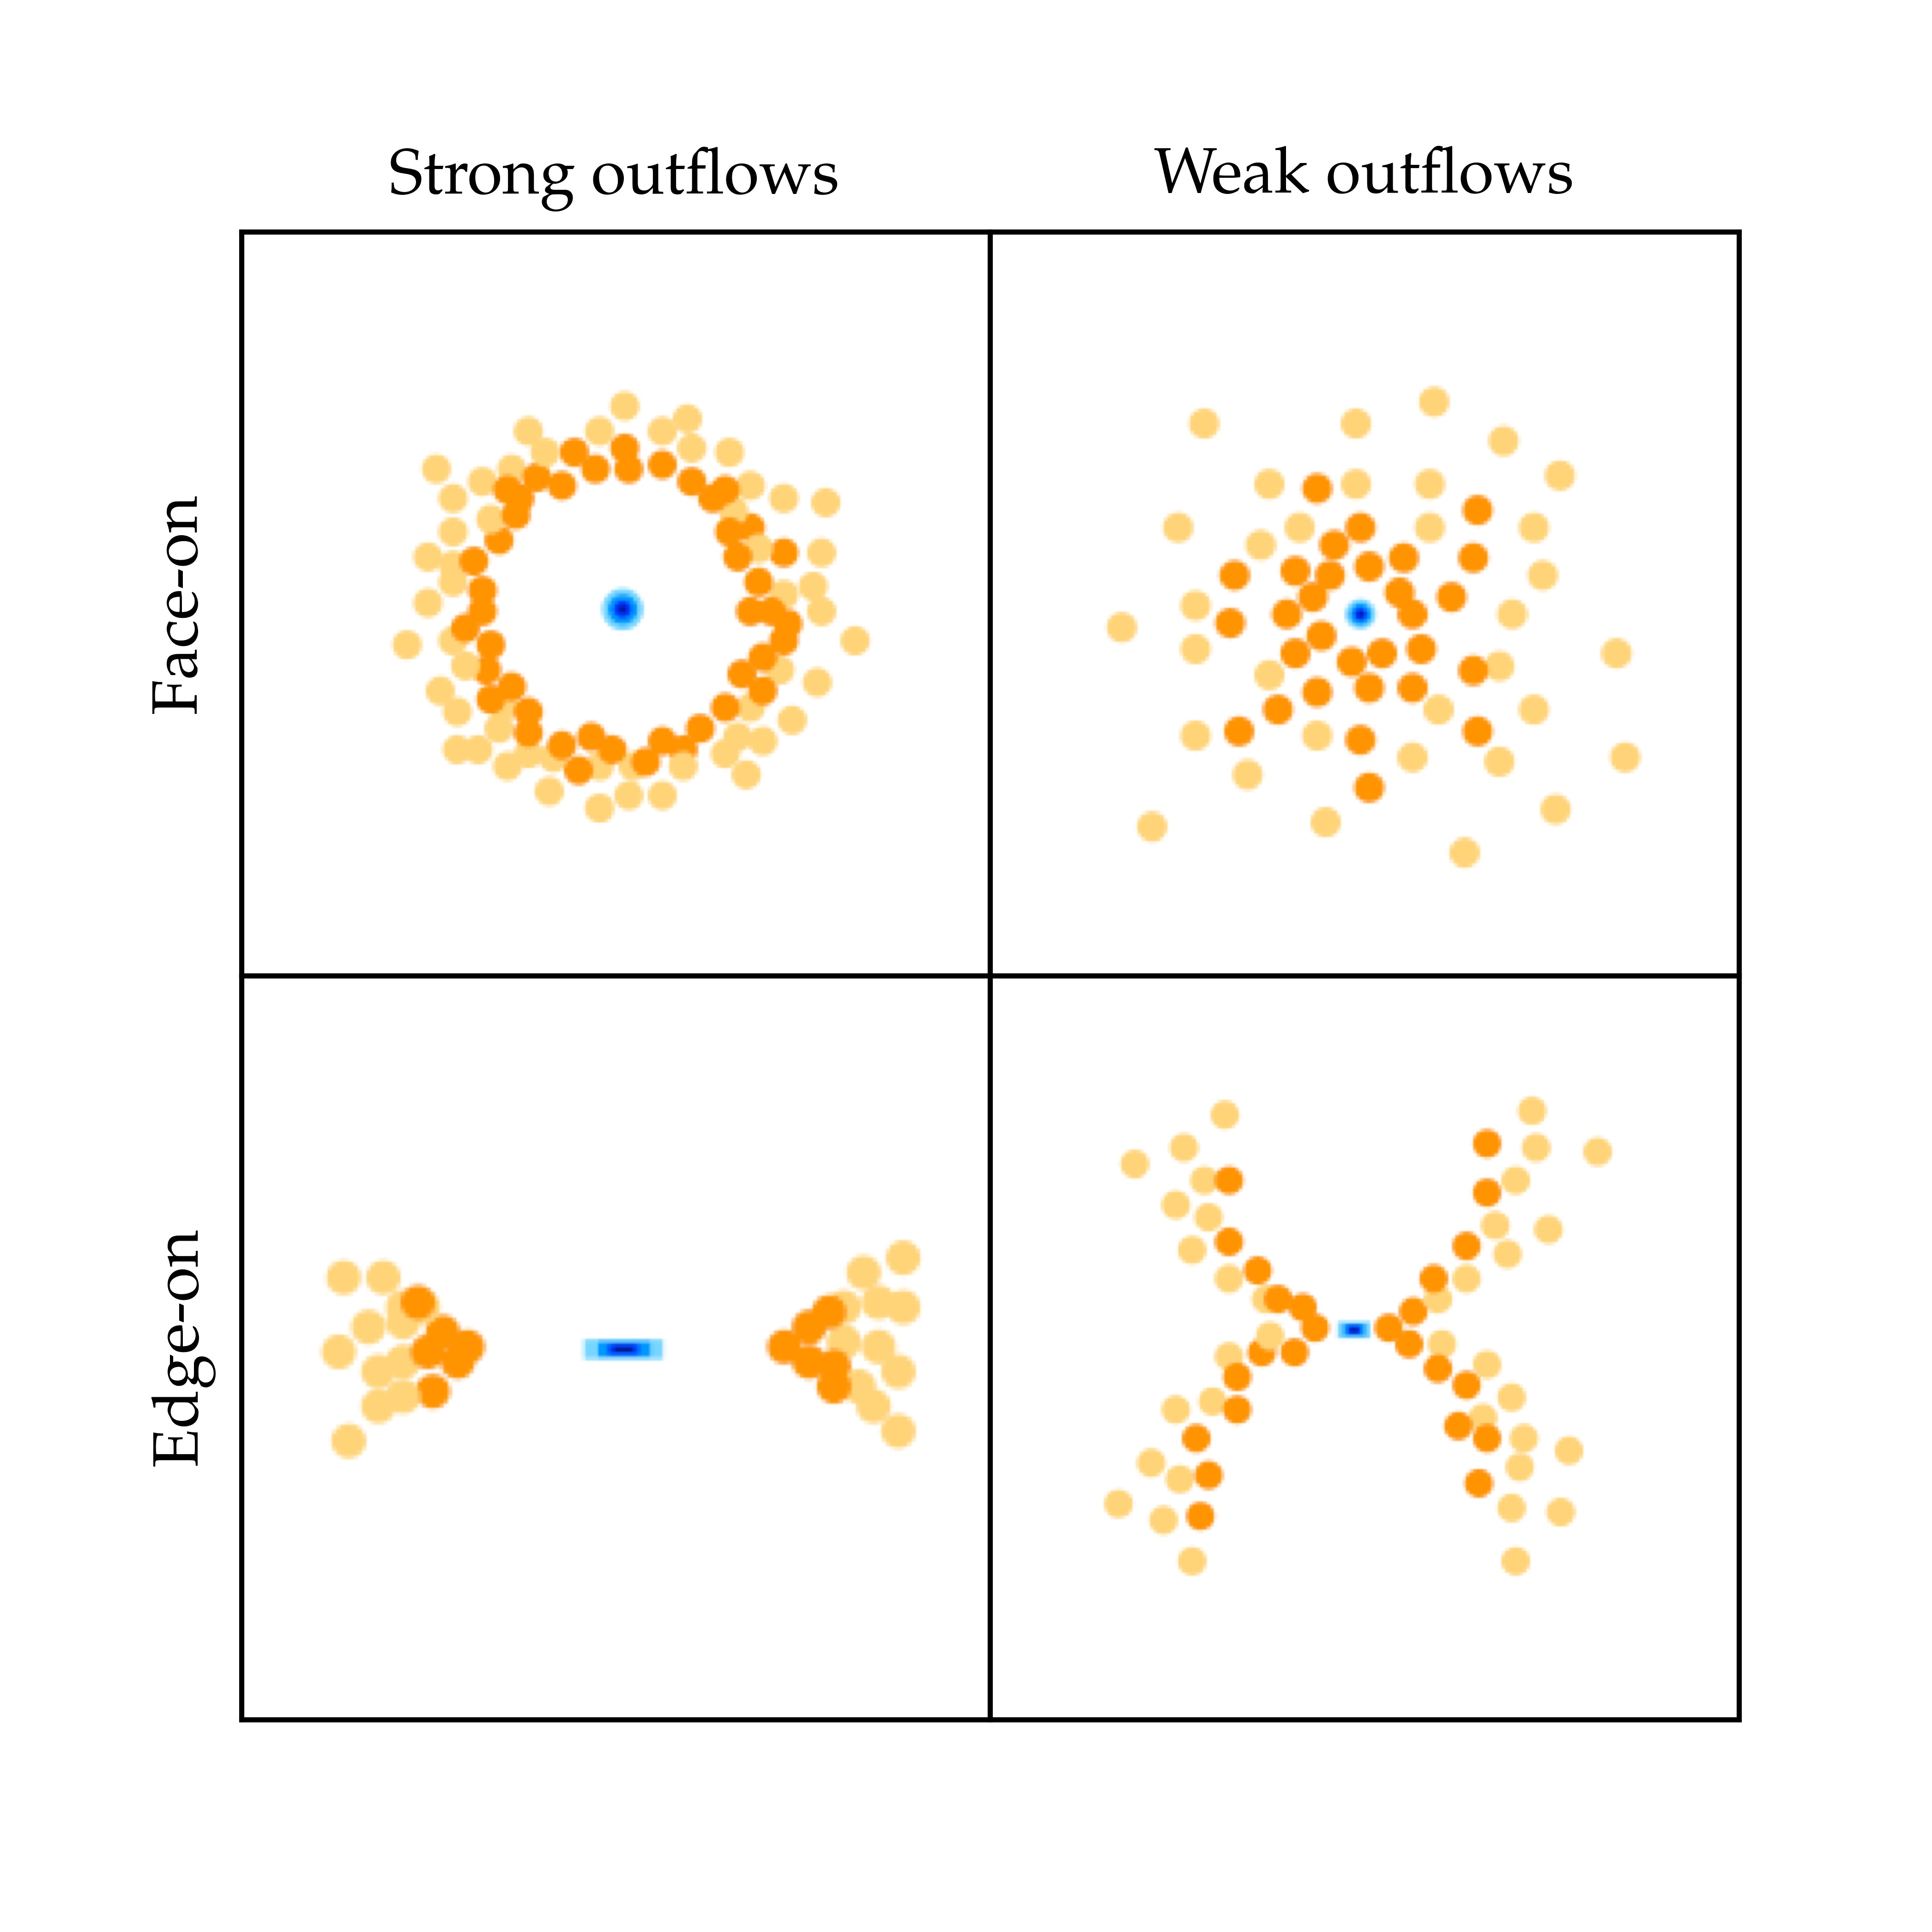
\includegraphics[width=1.0\textwidth]{figures/chapter05/kishimoto.jpg}
\caption[{Illustration of torus wind model.}]{Illustration of torus wind model. Accretion disc photons accelerate the dusty wind and flatten its geometry. This exposes more of the inner edge of the base of the wind, thereby enhancing the observed hot dust emission. Such a model can explain the correlation between outflow and hot dust properties seen in Figure~\ref{fig:civ_hot_dust}. Image credit: M. Kishimoto.}
  \label{fig:kishimoto}
\end{figure}

\subsection{Correlations with fundamental quasar properties}

\begin{figure}
\captionsetup[subfigure]{labelformat=empty}
  \centering
  \subfloat[\label{fig:correlations_contour_a}]{}
  \subfloat[\label{fig:correlations_contour_b}]{}
  \subfloat[\label{fig:correlations_contour_c}]{}
  \subfloat[\label{fig:correlations_contour_d}]{}
  \subfloat[\label{fig:correlations_contour_e}]{}
  \subfloat[]{{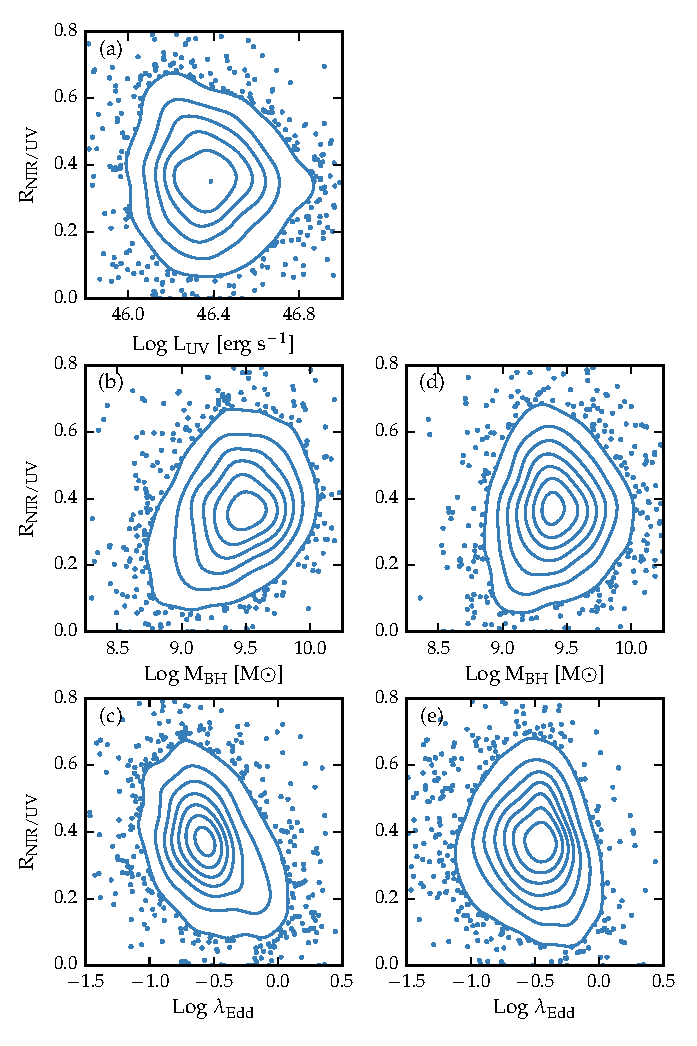
\includegraphics[width=\textwidth]{figures/chapter05/correlations_contour.pdf} }}
  \caption[{Best-fitting near-infrared to ultra-violet luminosity as a function of ultra-violet luminosity, BH mass and Eddington ratio.}]{Best-fitting near-infrared to ultra-violet luminosity ($R_{\text{NIR/UV}}$) as a function of ultra-violet luminosity, BH mass and Eddington ratio. In (b) and (c) BH mass estimates are taken from \citet{shen11}. In (d) and (e) BH mass estimates have been corrected using the procedure described in Chapter~\ref{ch:bhmass}. Using the corrected masses the correlations between $R_{\text{NIR/UV}}$ and the BH mass and Eddington ratio are significantly reduced.}
  \label{fig:correlations_contour}
\end{figure}

In this section, we look for correlations between the hot dust abundance, $R_{\text{NIR/UV}}$, and the ultra-violet luminosity, BH mass and Eddington ratio.

In Figure~\ref{fig:correlations_contour_a} we show $R_{\text{NIR/UV}}$ as a function of the ultra-violet luminosity.
The ultra-violet luminosity, which is measured at $1350$\,\AA, is reported in the catalogue of SDSS spectral properties from \citet{shen11}.
We do not observe any correlation between $R_{\text{NIR/UV}}$ and the ultra-violet luminosity (Figure~\ref{fig:correlations_contour_a}).
However, the dynamic range in luminosity is small ($\sim1$\,dex) because of the restricted redshift range.

In Figure~\ref{fig:correlations_contour_b} we show $R_{\text{NIR/UV}}$ as a function of the BH mass.
Masses are \ion{C}{IV} FWHM-based single-epoch virial estimates, as computed by \citet{shen11}.
$R_{\text{NIR/UV}}$ is positively correlated with the BH mass ($\rho_{\text{S}} = 0.26$; p-value $=6\times10^{-26
}$).
However, in the previous section, we found $R_{\text{NIR/UV}}$ to be correlated with the \ion{C}{IV} blueshift and, in Chapter~\ref{ch:bhmass}, we demonstrated that BH masses are severely overestimated in quasars with large \ion{C}{IV} blueshifts.
We therefore predict that the apparent correlation between $R_{\text{NIR/UV}}$ and the BH mass is due to systematic biases in the \ion{C}{IV}-based masses that are correlated with the \ion{C}{IV} blueshift.
We can test this by comparing $R_{\text{NIR/UV}}$ with BH mass estimates which have been corrected using the prescription described in Chapter~\ref{ch:bhmass} (Figure~\ref{fig:correlations_contour_d}).
As predicted, the correlation is significantly reduced ($\rho_{\text{S}}=0.07$; p-value $=2\times10^{-3}$).
A similar result is found when $R_{\text{NIR/UV}}$ is compared to the Eddington ratio, which is inversely proportional to the BH mass.
Using un-corrected masses from \citet{shen11} an anti-correlation is observed between $R_{\text{NIR/UV}}$ and the Eddington ratio ($\rho_{\text{S}}=-0.36$; p-value $=4\times10^{-51}$; Figure~\ref{fig:correlations_contour_c}) but this disappears when un-biased masses are employed ($\rho_{\text{S}}=-0.12$; p-value $=1\times10^{-10}$; Figure~\ref{fig:correlations_contour_e}).
This demonstrates how using conventional BH mass estimates based on \ion{C}{IV} can lead to spurious correlations with other quasar properties that are correlated with the \ion{C}{IV} blueshift, but that this can be avoided using the un-biased mass estimates presented in Chapter~\ref{ch:bhmass}.

\section{Summary}

The main results for this chapter are as follows:

\begin{itemize}

\item Using data from a number of recent wide-field photometric surveys, we build a parametric SED model that is able to reproduce the median optical to infrared colours of tens of thousands of SDSS AGN at redshifts $1 < z < 3$.

\item In individual objects, we find significant variation in the near-infrared SED dominated by emission from hot dust. We find the hot dust abundance to be strongly correlated with the strength of outflows in the quasar BLR, suggesting that the hot dust may be in a wind emerging from the outer edges of the accretion disc.



\end{itemize}
